\documentclass[a4paper]{article}

%% Language and font encodings
\usepackage[english]{babel}
\usepackage[utf8x]{inputenc}
\usepackage[T1]{fontenc}
\usepackage{listings}
\usepackage{minted}

%% Sets page size and margins
\usepackage[a4paper,top=3cm,bottom=2cm,left=3cm,right=3cm,marginparwidth=1.75cm]{geometry}

%% Useful packages
\usepackage{amsmath}
\usepackage{graphicx}
\usepackage[colorinlistoftodos]{todonotes}
\usepackage[colorlinks=true, allcolors=blue]{hyperref}

\title{Traveling Salesman Problem}
\author{Khalid Hourani}

\begin{document}
\maketitle

\noindent The Traveling Salesman Problem:

\indent Given a list of cities and a the distance between any two cities, what is the shortest route that visits each city exactly once and returns to the original city?

This can be visualized as a Graph Problem by creating an undirected, weighted graph in which the cities are represented by vertices and the distances are represented by weighted edges. For example, consider the following cities and distances:

\begin{center}\begin{tabular}{|c|c|c|c|c|c|c|}\hline \text{City} &C1 &C2&C3&C4&C5&C6\\\hline C1 & 0 & 3 & 4 & 4 & 10 & 10\\\hline C2 & 3 & 0 & 1 & 10 & 6 & 7\\\hline C3 & 4 & 1 & 0 & 9 & 6 & 6\\\hline C4 & 4 & 10 & 9 & 0 & 4 & 4 \\\hline C5& 10 & 6 & 6 & 4 & 0 & 8\\\hline C6& 10 & 7 & 6 & 4 & 8 & 0\\\hline\end{tabular}\end{center}

This can be represented with the following undirected, weighted graph:

\begin{center}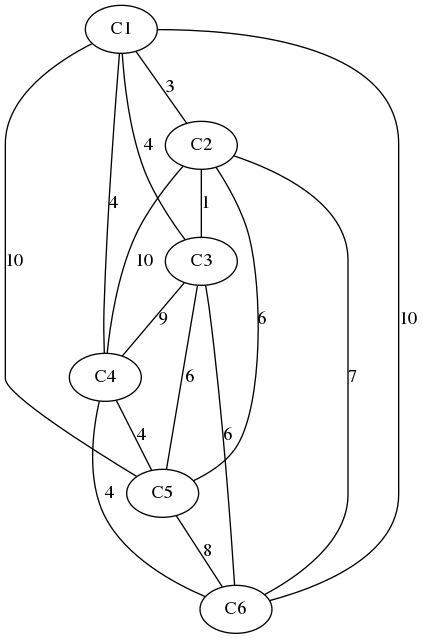
\includegraphics[scale=0.25]{graph.png}\end{center}

A brute-force search of all possible paths shows that the shortest distance is given by traveling in the following order: 

\[1 \to 2 \to 3 \to 5 \to 6 \to 4\]

For a graph with $n$ vertices and edges, there are $n!$ possible routes. This means that, as the number of cities increases, a brute-force search of all possible routes becomes unfeasible. In fact, with $n=20$, there are $20!=2432902008176640000\approx2.4\times10^{18}$ possible routes to search. 

\end{document}
